\documentclass[10pt,a4paper]{article}
\usepackage[utf8]{inputenc}
\usepackage{amsmath}
\usepackage{amsfonts}
\usepackage{amssymb}
\usepackage{graphicx}
%\author{Thomas Fuller}
\title{PD Controller Design}
\usepackage{hyperref}
\hypersetup{
    colorlinks=true,
    linkcolor=blue,
    filecolor=magenta,
    urlcolor=cyan,
}



\begin{document}
\maketitle
\section*{Introduction}
Practice problems so you guys can do for our exam. For each of the following systems which are in negative unity feedback, perform the following tasks.
\\ \\ 
1. Evaluate the Routh Hurwitz Criterion to determine a stable range of ``K" for the system.
\\ \\ 
2.  Sketch the root locus using the steps we talked about in class. Sketch it, but you will also need to use the \texttt{rlocus} command in order to do problem 3, so verify your sketch in MATLAB as well.
\\ \\
3.  Design a PD controller with the properties listed under each question, and plot the initial and final responses, verifying the design.
\section{First Plant}
This first one is just to warm us up and we did it in class.
\begin{equation*}
G(s) = \frac{K}{s(s+4)(s+6)}
\end{equation*}
Design the P.D. Controller to have 16\% overshoot, and reduce the settling time by 3x.  
\section{Second Plant}
\begin{equation*}
G(S) = \frac{K}{s(s+8)(s+25)}
\end{equation*}
Design the P.D. Controller to have 20.5 \% overshoot, and reduce the settling time by a factor of 4. 
\section*{Root Locus}
Write the open loop transfer function if the root locus is taken of a systme in unity feedback. 
\\ \\
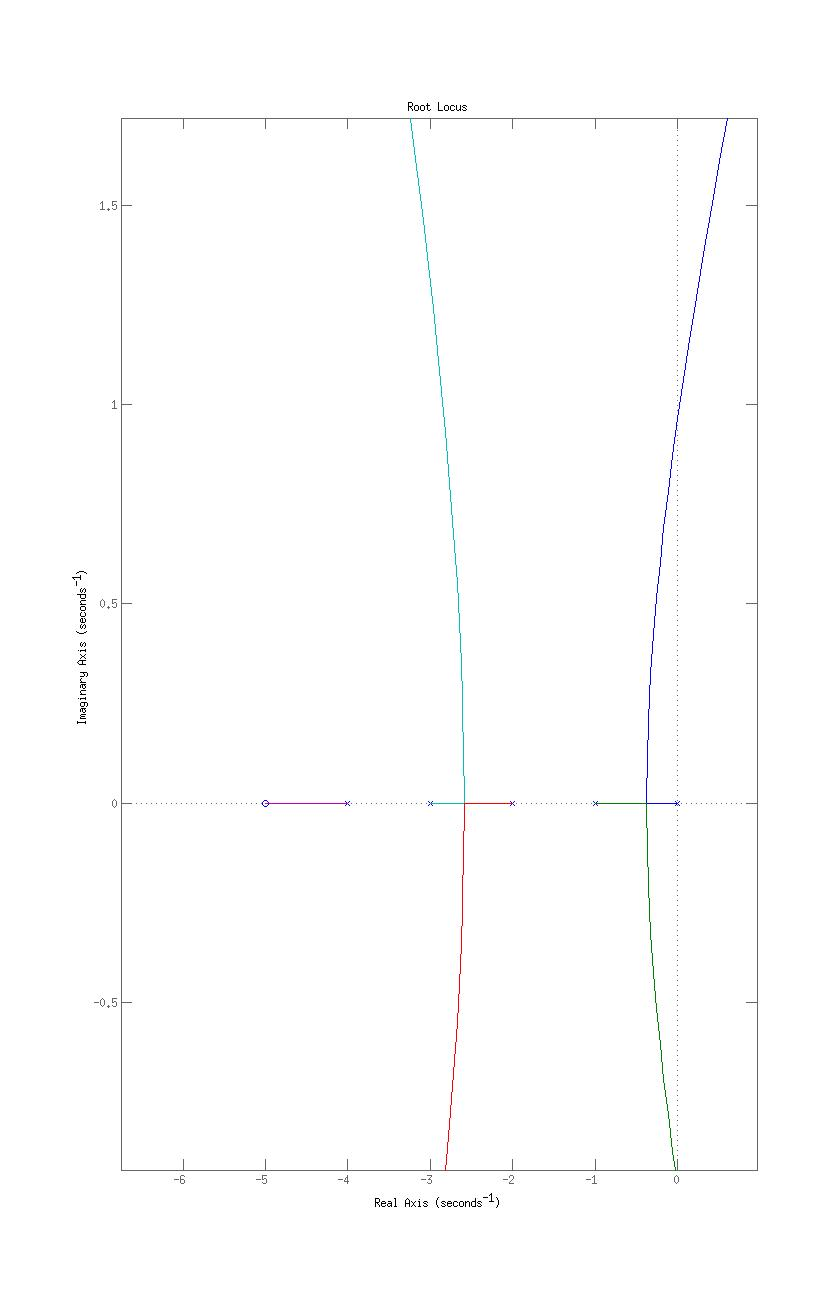
\includegraphics[scale=0.4]{rootlocus.jpg}
\section*{Inspirational Quote}
You can do it!
\end{document}
